
\documentclass{knac}

% This next line is only necessary to get a live hyperlink in the
% output document:
\usepackage{natbib}
\usepackage{hyperref}
\usepackage{gensymb}
\usepackage{tabu, booktabs}


%  If you want to define shortcuts for commonly-typed commands you'll
%  use, you can do so here - for example, here is a command to make it
%  easier to refer to H alpha emission (using 'math mode', denoted by
%  the dollar signs, to generate the Greek letter alpha).

\newcommand{\ha}{H$\alpha$}


\begin{document}

% Give the title of the paper here.
\title{Modelling the Kinematics of HD 100546: ALMA Evidence for a Planetary Companion?}

% Don't use the AASTeX-style commands \affil, \email, etc. for
% specifying various parts of the author or advisor information here -
% just give the author(s) and affiliation(s) just as you would like
% them to appear in the document:

\author{Cail Daley, Wesleyan University}

% If there are multiple advisors, use \advisors instead.
\advisor{Catherine Walsh, Leiden University and University of Leeds}


\begin{abstract}
  HD 100546 is a nearby Herbig Be star surrounded by an early-stage transition disk. This disk is known to have a complex physical structure, and hosts a confirmed protoplanet at \textasciitilde 53 AU with a possible second companion at \textasciitilde 14 AU. We model the velocity structure of the CO ($J=3-2$) line emission in the disk to compare with ALMA data and find the disk to be much flatter than previously expected. Modeling also reveals significant super-Keplerian velocities in the inner regions of the disk, possibly stemming from a dust-trap-induced vortex or a circumplanetary disk. Three components are needed to reproduce the observed velocity structure: a basic Keplerian velocity field with a position angle of 144\textdegree \ and inclination of 36\textdegree, a warped inner disk with position angle of 75\textdegree \ and inclination of 64\textdegree, and a non-axisymmetric ``blob'' of super-Keplerian gas.

\end{abstract}

% After this comes your document.  You can use section headings with
% the \section command.  (And also \subsection if you wish.)

\section{Introduction}
Young (<10 Myr old) stars are often surrounded by circumstellar disks, huge rotating reservoirs of gas and dust left over from the process of star formation that are responsible for the genesis of nearly all of the known asteroids, comets, and planets in the universe. As dust grains in circumstellar disks collide and stick together, they can form larger bodies known as planetesimals, which can in turn grow large enough to exert significant gravitational attraction on the material surrounding them. Gas and dust fall towards such ``protoplanets'' in a process known as accretion, occasionally forming circumplanetary disks within the surrounding circumstellar environment. Planets can have significant effects on the structure of their parent circumstellar disks, for example clearing gaps or launching spiral density waves and vortices (\citealt{Baruteau13}). Such planet-disk interactions provide scientists with a useful tool in planet detection, allowing them to infer the presence of unseen planets from the structure of the surrounding circumstellar disk. \\
\indent HD 100546, a nearby Herbig B9V Be star surrounded by an early-stage transition disk, presents a promising opportunity to explore such relationships. The presence of a $~5M_{Jup}$ protoplanet at ~53 AU has been confirmed, and there is evidence for an older $10-20 M_{Jup}$ protoplanetary companion at ~14 AU (\citealt{Quanz15, Currie15,Pinilla15}). This rich planetary environment is complemented by a complex disk structure complete with spiral arms and rings as well as several other unusual features (\citealt{Grady05, Boccaletti13, Walsh14}). The abundance of protoplanets and structural features in HD 100546's disk, as well as its proximity, distinguish the system as a particularly interesting location to study planet-disk interactions.

\begin{figure}
  \label{fig:moment}
  \centering
  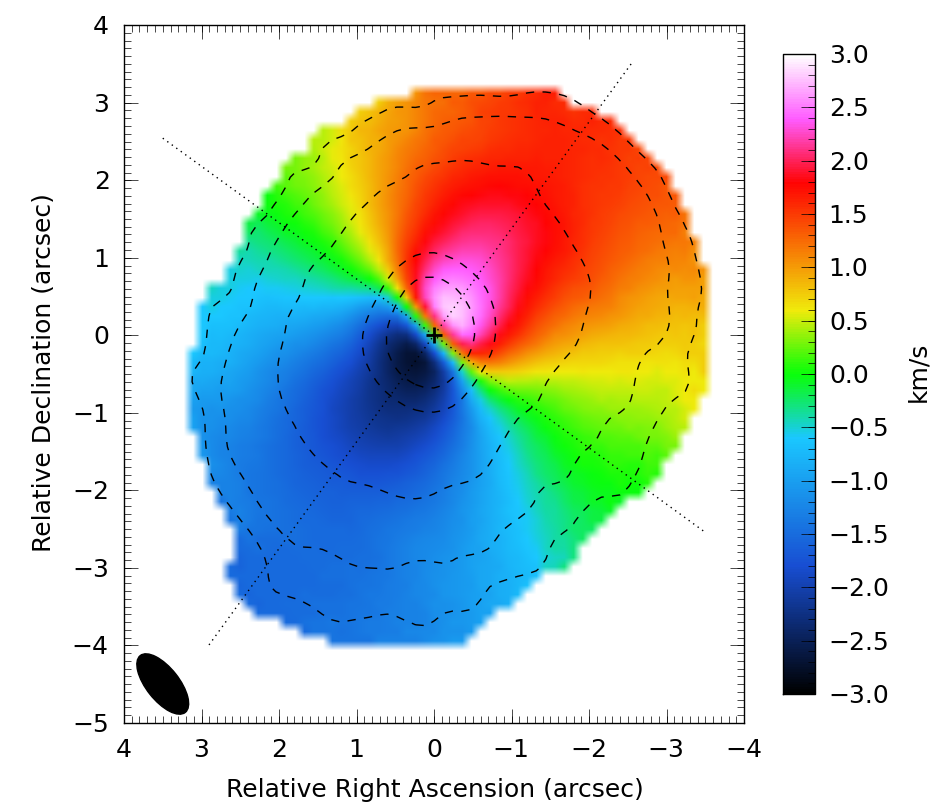
\includegraphics[width=12 cm]{moment0.png}
  \caption{First moment map of HD 100546's disk traced in line emission from CO $(J=3-2)$. The disk is rotating counterclockwise, with the lower left part of the disk blueshifted towards the observer and the upper right redshifted away. The gas with the same radial component as the star lies along the semi-minor axis of the disk, parallel to the observer's line of sight. The image has a beam size (spatial resolution) of 0.94" x 0.42".}
\end{figure}

\section{Methods \& Analysis}
The data used in this paper were taken on November 18, 2012 as part of ALMA Cycle 0 (program 2011.0.00863.S, P.I. C. Walsh). Observations made use of 24 antennas with baseline lengths ranging between 21 m and 375 m, and were taken at 300 and 345 Ghz with velocity resolutions of 0.24 and 0.21 km/s respectively. For further details, see \cite{Walsh14}.\\
\indent In order to gain information about HD 100546's disk, we modeled the velocity structure of the carbon monoxide (CO) $J=3-2$ emission; Figure 1 displays the first moment map (intensity-weighted velocity distribution) of the CO in the disk. We extended the functionality of a code written by Catherine Walsh and Atilla Juhasz, which, when given a set of input parameters, analytically generates a Keplerian velocity field that can then be compared to the observed first moment map. Stellar mass was fixed at $2.4M_{\odot}$, and the distance was fixed at 96.9 parsecs (\citealt{Ancker98, Meeus12}); all other parameters were varied. For each combination of parameters, a sum-of-squares fit statistic was calculated. The best-fit model was then determined by finding the global minimum of a ``grid'' of these fits bounded by the parameter ranges found in Table 1.\\
\indent The first iteration of our model was a simple Keplerian velocity field as described above. In this round of modeling, values for position angle ($\phi$), inclination ($i$), cone aspect ratio, and cone face were allowed to range within the bounds described in Table 1. Aspect ratio is the ratio of disk scale height ($z$) to radius ($r$) for any given $r$. Cone face is only relevant for a non-flat disk, i.e. $\frac{z}{r} > 0$, and describes whether the ``upper'' or ``lower'' face of the disk's double cone is closer to the observer.\\
\indent A simple Keplerian velocity field fits the outer regions of the disk quite well; however, in the inner regions of the disk the model under-predicts the data by over 1.5 km/s, as seen in Figure 2(a). In order to better reproduce the data, we added a second component to the model, an inner warp. In a warped disk, part of the disk has a different position angle and/or inclination; if the inner regions of HD 100546's disk were warped to a higher inclination, the observed velocities would be higher than those predicted by a purely Keplerian model. The position angle and inclination of the outer disk were fixed to the best fits of the basic model, while the position angle, inclination, and transition radius of the inner disk were allowed to vary. The warp model was able to reproduce the redshifted portion of the disk, but significant residuals remained on the blueshifted side; this made it clear that the velocity structure could not be fit by an axisymmetric model.\\
\indent In order to reproduce the non-axisymmetric, super-Keplerian ``blob'' visible in the residual map of Figure 2(b), we artificially increased the velocity within a wedge of the disk roughly corresponding to the size and orientation of the blob. Wedge start and end position angle,  outer radius, and velocity were all allowed to vary. This ``blob'' model was able to account for the super-Keplerian velocities on the blueshifted side of the disk, but the residuals on the redshifted side of the disk that had been removed by the warp model reappeared. This led us to conclude that neither a blob nor warp model alone could reproduce HD 100546's velocity structure, and that both the blob and warp models must be stacked with the basic Keplerian model. Due to the number of parameters and spatial resolution limits of the data, parameters were not allowed to vary; instead, a fit by eye technique was used to gain a qualitative understanding of the disk's velocity structure. This three-component model fit the data well, with most of the first moment map residuals falling within one velocity resolution (0.22 km/s) of the source velocity.


\begin{table}
\label{tab:parameters}
\centering
\begin{tabu}{X[l]X[c]X[c]}
  \toprule
Parameter 	&	Range&	 Preferred Value\\
\midrule
\textbf{Flat Model} & & \\
Position Angle &	[130,160]\degree   &	 144\degree\\
Inclination    &	[30,60]\degree	& 36\degree \\
Aspect Ratio   &	[0,0.5]   &	 0.02\\
Cone           &	[Lower, Upper] &	 Lower\\
\midrule
\textbf{Warp Model} & & \\
Transition Radius &	[20,90] AU   &	 40 AU\\
Inner Disk Position Angle &	[130,160]\degree	& 75\degree\\
Inner Disk Inclination    &	[30,60]\degree	& 64\degree \\
\midrule
\textbf{Blob Model} & & \\
Velocity     &  [-5, -15]km/s & -5 km/s\\
Outer Radius &	[30,100] AU   &	 80 AU\\
Start PA &	[9, 44]\degree	& 39\degree\\
End PA &	[44,84]\degree	& 69\degree \\
\midrule
\textbf{Blob + Warp Model} & & \\
Warp Radius & & 40 AU\\
Warp PA & & 114\degree\\
Warp Inclination & & 56\degree\\
Blob Velocity     &  & -8.2 km/s\\
Blob Outer Radius &	 &	 65 AU\\
Blob Start PA & & 44\degree\\
Blob End PA &	& 74\degree \\
\bottomrule
\end{tabu}
\caption{HD 100546 Parameters \& Best Fits}
\end{table}

\begin{figure}
  \label{fig:model summary}
  \centering
  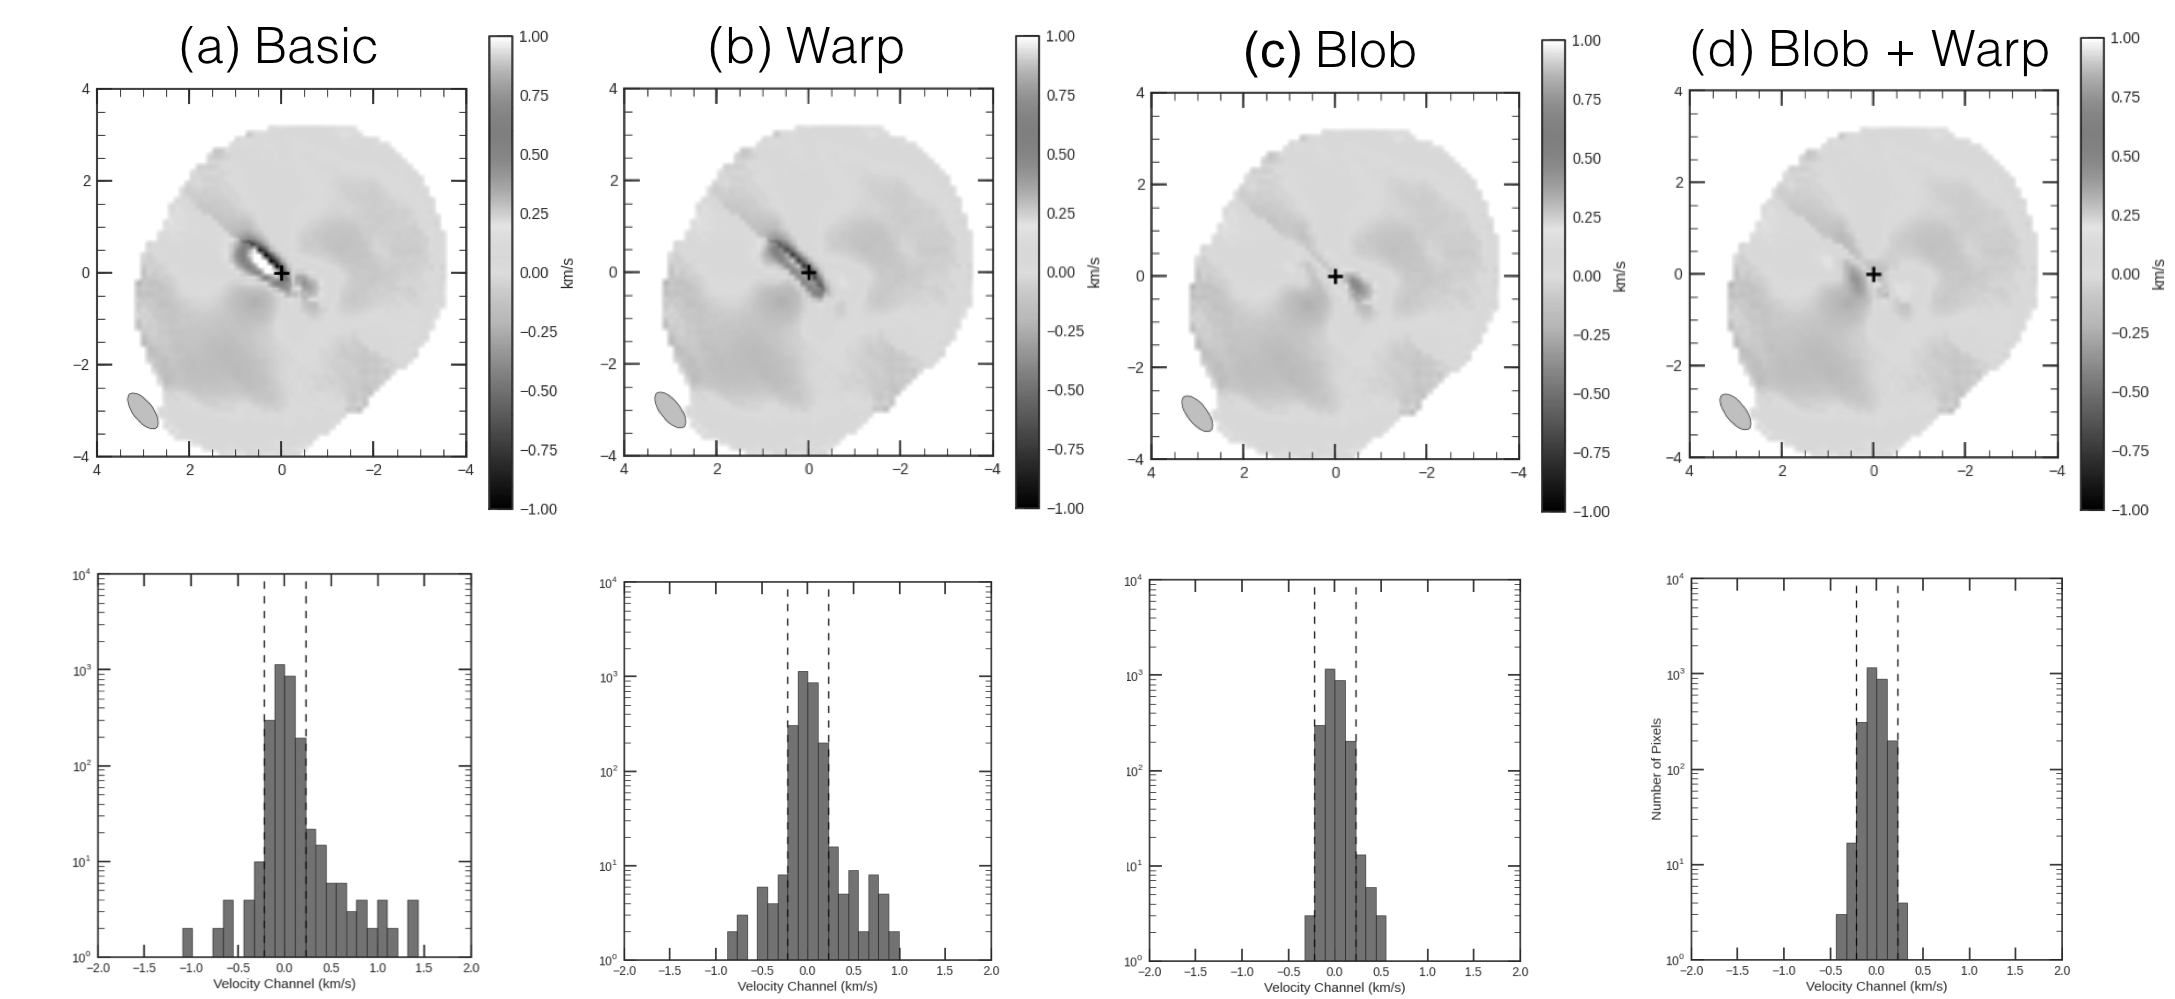
\includegraphics[width=\linewidth]{model_summary.png}
  \caption[No Warp Fit Plots]{Evolution of the model over time. The top row contains model residuals, and the bottom row contains a histogram of the residual pixels. The residual ``blob'' can seen above and left of the stellar location, which is marked with a `+,' in the residual map of panel (a). The warp model of panel (b) eliminates the redshifted residuals to the right of the star, and the blob model (panel c) eliminates the blueshifted residuals to the right of the star only to reintroduce the redshifted residuals. Panel (d) shows the final best-fit model with no significant residuals.}
\end{figure}


\section{Results \& Discussion}

Three different model components are needed to fit the velocity distribution of the CO in HD 100546's disk: a basic Keplerian velocity field, a warped inner disk, and a non-axisymmetric ``blob.'' Parameter information, including best fits, can be found in Table 1. It is important to note that although the individual models are well constrained, degeneracies are likely in the combined blob and warp model due to the spatial resolution of the data. \\
\indent The preferred aspect ratio, corresponding to a height angle of only 1 degree, indicates that the CO(3-2) emitting layer lies remarkably close to the midplane of the disk. This suggests that HD 100546 belongs to  group II of Herbig Ae/Be stars, characterized by flat, unflared disks. This is in conflict with \cite{Meeus01}'s classification of the disk as group I, associated with thick and highly flared disks, based on its spectral energy distribution.\\
\indent There are several possible explanations for the super-Keplerian, non-axisymmetric ``blob'' in the inner regions of HD 100546's disk. A dust trap could create a vortex on the blueshifted side of the disk, locally increasing velocities of the carbon monoxide; however, no evidence for a dust trap has been found (M. Kama, private communication). It also is possible that the observed super-Keplerian velocities are produced by a circumplanetary disk, possibly surrounding the protoplanet candidate at 14 AU. If the candidate were accompanied by such a disk and were in the plane of the best-fit warp model ($i=64\degree$), the observed gas velocities would be roughly 18 km/s. As the spatial resolution of the data is 11 AU, and a 20 $M_{Jup}$ protoplanet at 14 AU could harbor a circumplanetary disk with a radius of up to 2 AU, it is possible that the excess velocity stems from only one pixel and is ``smeared'' to a greater spatial extent by the restoring beam. The hypothesis of an unresolved source is further supported by the fact that the residual blob is roughly the same size and orientation as the beam itself. However, the spatial resolution of the data is not high enough to arrive at definite conclusions as to the nature of the blob, other than that three model components are needed to fit the data. Higher spatial resolution observations are needed to interpret the physical significance of HD 100546's velocity structure, but findings such as these suggest that features on the scale of planets and their disks may soon lie at the frontier of sub-millimeter radio astronomy.




% Give the acknowledgments here.  Citing the NSF grant that funds the
% REU program is a good idea (just using the text below).  In the
% interest of saving space, there is no section heading inserted here
% specifically for acknowledgments.

\acknowledgments

I would like to thank my supervisors Catherine Walsh and Paola Pinilla for the encouragement, kindness, and advice that allowed this project to be both challenging and legitimately fun. I am also grateful for my roommate and colleague Shreyas Vissapragrada, as well as my academic advisor Meredith Hughes.
We gratefully acknowledge Leiden University for making this research opportunity possible. This paper makes use of the following ALMA data: ADS/JAO.ALMA\#2011.0.00863.S.



% Here's how we specify the bibliography.

\bibliographystyle{plainnat}
\bibliography{KNAC}

% For including references in the final reference list, you can get
% Latex-formatted references directly from NASA ADS
% (http://www.adsabs.harvard.edu/abstract_service.html) - after
% finding the reference you want, click on "Preferred format for this
% abstract" and you will get a \bibitem record in Latex format that
% can be pasted in your document.

% Note that each bibitem record has three parts: the first part in
% curly braces is how the citation will appear in the text; the second
% is a shorthand tag that you use to refer to the paper by name; and
% the third is the contents of the bibliography entry.  Leave the
% first and third parts alone, but you can edit the second part (in
% square braces) to be whatever abbreviation you want to use to refer
% to that paper - here I've changed the default ones that come from
% ADS to be something I can remember more easily (usually just an
% author and year).  These are the tags that are used above in the
% \citet and \citep commands.


% \bibitem[Willman
% \& Strader(2012)]{Willman2012} Willman, B., \& Strader, J.\ 2012, \aj, 144, 76



\end{document}
